\documentclass[12pt]{article}

\usepackage{amsthm,amsmath,amssymb,amsfonts}
\usepackage{tikz}
\usepackage[utf8]{inputenc}
\usepackage[T1]{fontenc}
\usepackage{babel}
\usepackage{graphicx}
\usepackage{listings}
\usepackage{multirow}
\usepackage{fancyhdr}
\usepackage{tocbibind}
\usepackage{lmodern}
\usepackage{color}
\usepackage{geometry}
\usepackage{hyperref} %Sert à utiliser la commande \href
\usepackage{listings} %Sert à introduire du code dans le fichier tex avec \begin{lstlisting} CODE \end{lstlisting}



%%%%%Marges & en-t\^etes

\geometry{hmargin=2.3cm, vmargin=3cm}
\fancyhf{} % supprime les en-tetes et pieds prédéfinis
\fancyhead[FC]{\bfseries\thepage} % N∞page centre bas
\fancyhead[HC]{\footnotesize\leftmark} % chapitre centre haut
\renewcommand{\headrulewidth}{0.2pt} % filet en haut
\addtolength{\headheight}{0.5pt} % espace pour le filet
\renewcommand{\footrulewidth}{0.2pt} %filet en bas




\newtheorem{theorem}{{\bf Théorème}}[section]
\newtheorem{assumption}[theorem]{Assumption}
\newtheorem{corollary}{{\bf Corollaire}}[section]
\newtheorem{lemma}{{\bf Lemme}}[section]
\newtheorem{proposition}{{\bf Proposition}}[section]
\newtheorem{definition}{{\bf Définition}}[section]
\textwidth = 16.5cm
\textheight = 21.3cm
\topmargin = 0.cm
\evensidemargin = 0.cm
\oddsidemargin = 0.cm


%%\renewcommand{\theequation}{{\rm\thesection.\arabic{equation}}}

\begin{document}
\title{A quick overview about challenges \\  in Data Sciences and Blockchain}
\author{Thomas Suau}

\maketitle
\numberwithin{equation}{section}
\abstract{
The goal of this paper is to give a brief overview about how data knowledges can be used in Blockchain research. 


The goal is not to solve actuals problems only to give some research proposals in Blockchain and Data Sciences.

With recent developments over Bitcoin protocol \cite{BIP341} and ethereum scaling proposals with layer 2 \cite{eth2} data is massively arriving in the Blockchain. This will issue numbered of new problems and new challenges. 

I hope to clarify the answer about : how data and blockchain are related ?\\ 
%How to use data knowledge to understand several different blockchains and provide analysis about them ? 
%How to use storage offered in blockchains to develop ?\\
%Moreover what data are pertinent and what can we do with them ?  
I want to focus on what interesting problems can be delve into the topic of blockchain and data. As generally as possible.\\
To stay synthetic I kept 5 major challenges and I purpose a simplified plan to attack them. 
}

\newpage


\tableofcontents

\newpage 

\section{Introduction}


As we know data are today a core in major part of computer sciences. Without doing again the history of computer science the data is one of the key concept in information theory.
With the growth of computer capacities we are today able to store and manage huge amount of data. This is so called big data \cite{bigdata}. 
These data are from different forms and often stored in dedicated server. One very common language to request these data is \texttt{SQL} even though many new requesting technics appearing called \texttt{No-SQL} with Mongo DB\cite{mongodb}, Cassandra DB\cite{cassandradb}, GraphQL \cite{graphql} and many others \cite{nosql}.\\

In another hand, since 2008 there is a new technology deployed : the Bitcoin \cite{whitepaper-btc}, with in its core the blockchain. The blockchain technology allow us to share value across digital realm. With Ethereum in 2014 \cite{whitepaper-eth}, a new type of blockchain appeared : a decentralised application platform. 
The idea behind Ethereum is to get everyone access to a decentralised Virtual Machine (the Ethereum Virtual Machine \cite{kevm}). We can use the EVM if we are paying gas \cite{gas-eth} in ETH (the cryptocurrency associated to Ethereum Blockchain). 
The access to EVM means that we have access to an hardware and we can make action on this hardware.  

In this point of view, the blockchain technology allow us to share our hardware and to be paid for this. We are also able to execute code (more precisely bytecode \cite{bytecode-evm}) and store data into the EVM storage (please find the schema in Appendix \ref{evm}).\\

{\bf What are issues and challenges associated to those data ?} \\

This article assumes to give a brief overview about actual problem in data and blockchains. It wouldn't be exhaustive because of the complexity of the topic should drive us around deep research as shown in Deepa, Pham et alt. \cite{survey-bigdata-blockchain} : \\
"Despite many research efforts, we are not aware of any survey that comprehensively studies the applicability of blockchain for big data applications. Although the survey in \cite{scalability-blockchain} reviews blockchain for big data applications and challenges, it is very short and not updated since it has been published several years ago."

Data are still in a human unreadable format, difficult to query as assume in Prytarski, et alt. \cite{query} and \href{https://ec.europa.eu/digital-building-blocks/code/projects/EBSI}{European Blockchain Service Infrastructure (EBSI)} is far to be usable. 

Many developments should be done in this way and as it's assume in Deepa, Pham et alt. \cite{survey-bigdata-blockchain} : "Blockchain with its decentralization and security nature has the great potential to improve big data services and applications".



\section{State of the art}

The state of the art will be brief as the research in this field. There are not many qualitatives research around blockchain compare to challenges blockchain is facing.

There is Hassani, et alt. \cite{bigdata} published in 2018. This article important for this field, is not at the cryptography academic level.  There is a lack of technical aspect and no authors are doing computer sciences in their research field. It's mainly general purpose and blockchain is apparently misunderstood in this paper. We can confirm this by checking their link to explain what blockchain is from a confused picture in 2.1.
There is a book published in 2015 Handbook of digital currency \cite{book-blockchain-data}. This book is an aggregation of different authors and topics around blockchain and data. The main focus is rather finance than blockchain or data themselves. It's very large and not as specific as current challenges.  

There are many references about specific applications like data integrity in Lui, et alt. \cite{data-integrity}, securing trading data in Wai, et alt. \cite{data-trading-secure} , fraud detection in Kamisalic et alt. \cite{fraud-detection}  and others like in medical records in Liu, Lam et alt. \cite{data-med}  or supply chain in Wang, et alt. \cite{data-supplychain}. 

The only academic paper with approaches, challenges and future perspective is about Blockchain for Big Data in Deepa, Pham et alt. \cite{survey-bigdata-blockchain}. Unfortunately the article conclude with  "Despite many research efforts, we are not aware of any survey that comprehensively studies the applicability of blockchain for big data applications. Although the survey in \cite{scalability-blockchain} reviews blockchain for big data applications and challenges, it is very short and not updated since it has been published several years ago.".\\

A deeper analysis of Prytarski, et alt. \cite{query} should be done. Even though their experiment of SQL queries is very short, they provided a good bibliography in their state of the art that should be interesting to delve.\\

With the recent update of Ethereum client \texttt{geth} \cite{geth}, we are now able to make GraphQL\cite{graphql} queries. This is also a major new updates and we need to update scientific research according to this. 


What I'm purposing is to give another regard to the link between Data and Blockchain.\\


\section{Challenges}

\begin{enumerate}

\item {\bf Retrieve data stored on-chain}\\ 
There exist tools to make \texttt{SQL} request \href{https://aws.amazon.com/blogs/database/access-bitcoin-and-ethereum-open-datasets-for-cross-chain-analytics/}{Access Bitcoin and Ethereum open datasets for cross-chain analytics} provided by AWS.
The query processing on blockchain is still a challenge as assume in Przytarski, Stach, Gritti et alt. \cite{query} where they can only try some \texttt{SELECT} statement by migrating original Ethereum LevelDB in SQLite. Regarding the exponential  growth of the Ethereum blockchain, we need to think about other ways to do so. The creativity will be a big challenge too.\\
Recent updates in \texttt{geth} \cite{geth} client haven't been regarded so far by academic community and it can be a good starting point.\\
As an example of data in a blockchain you can find one Bitcoin transaction which contains the JSON file below (more details about this is given Appendix \ref{bitcoin}). 
\begin{figure}[h!]
  \centering
  \begin{minipage}[b]{0.5\textwidth}
    \centering
    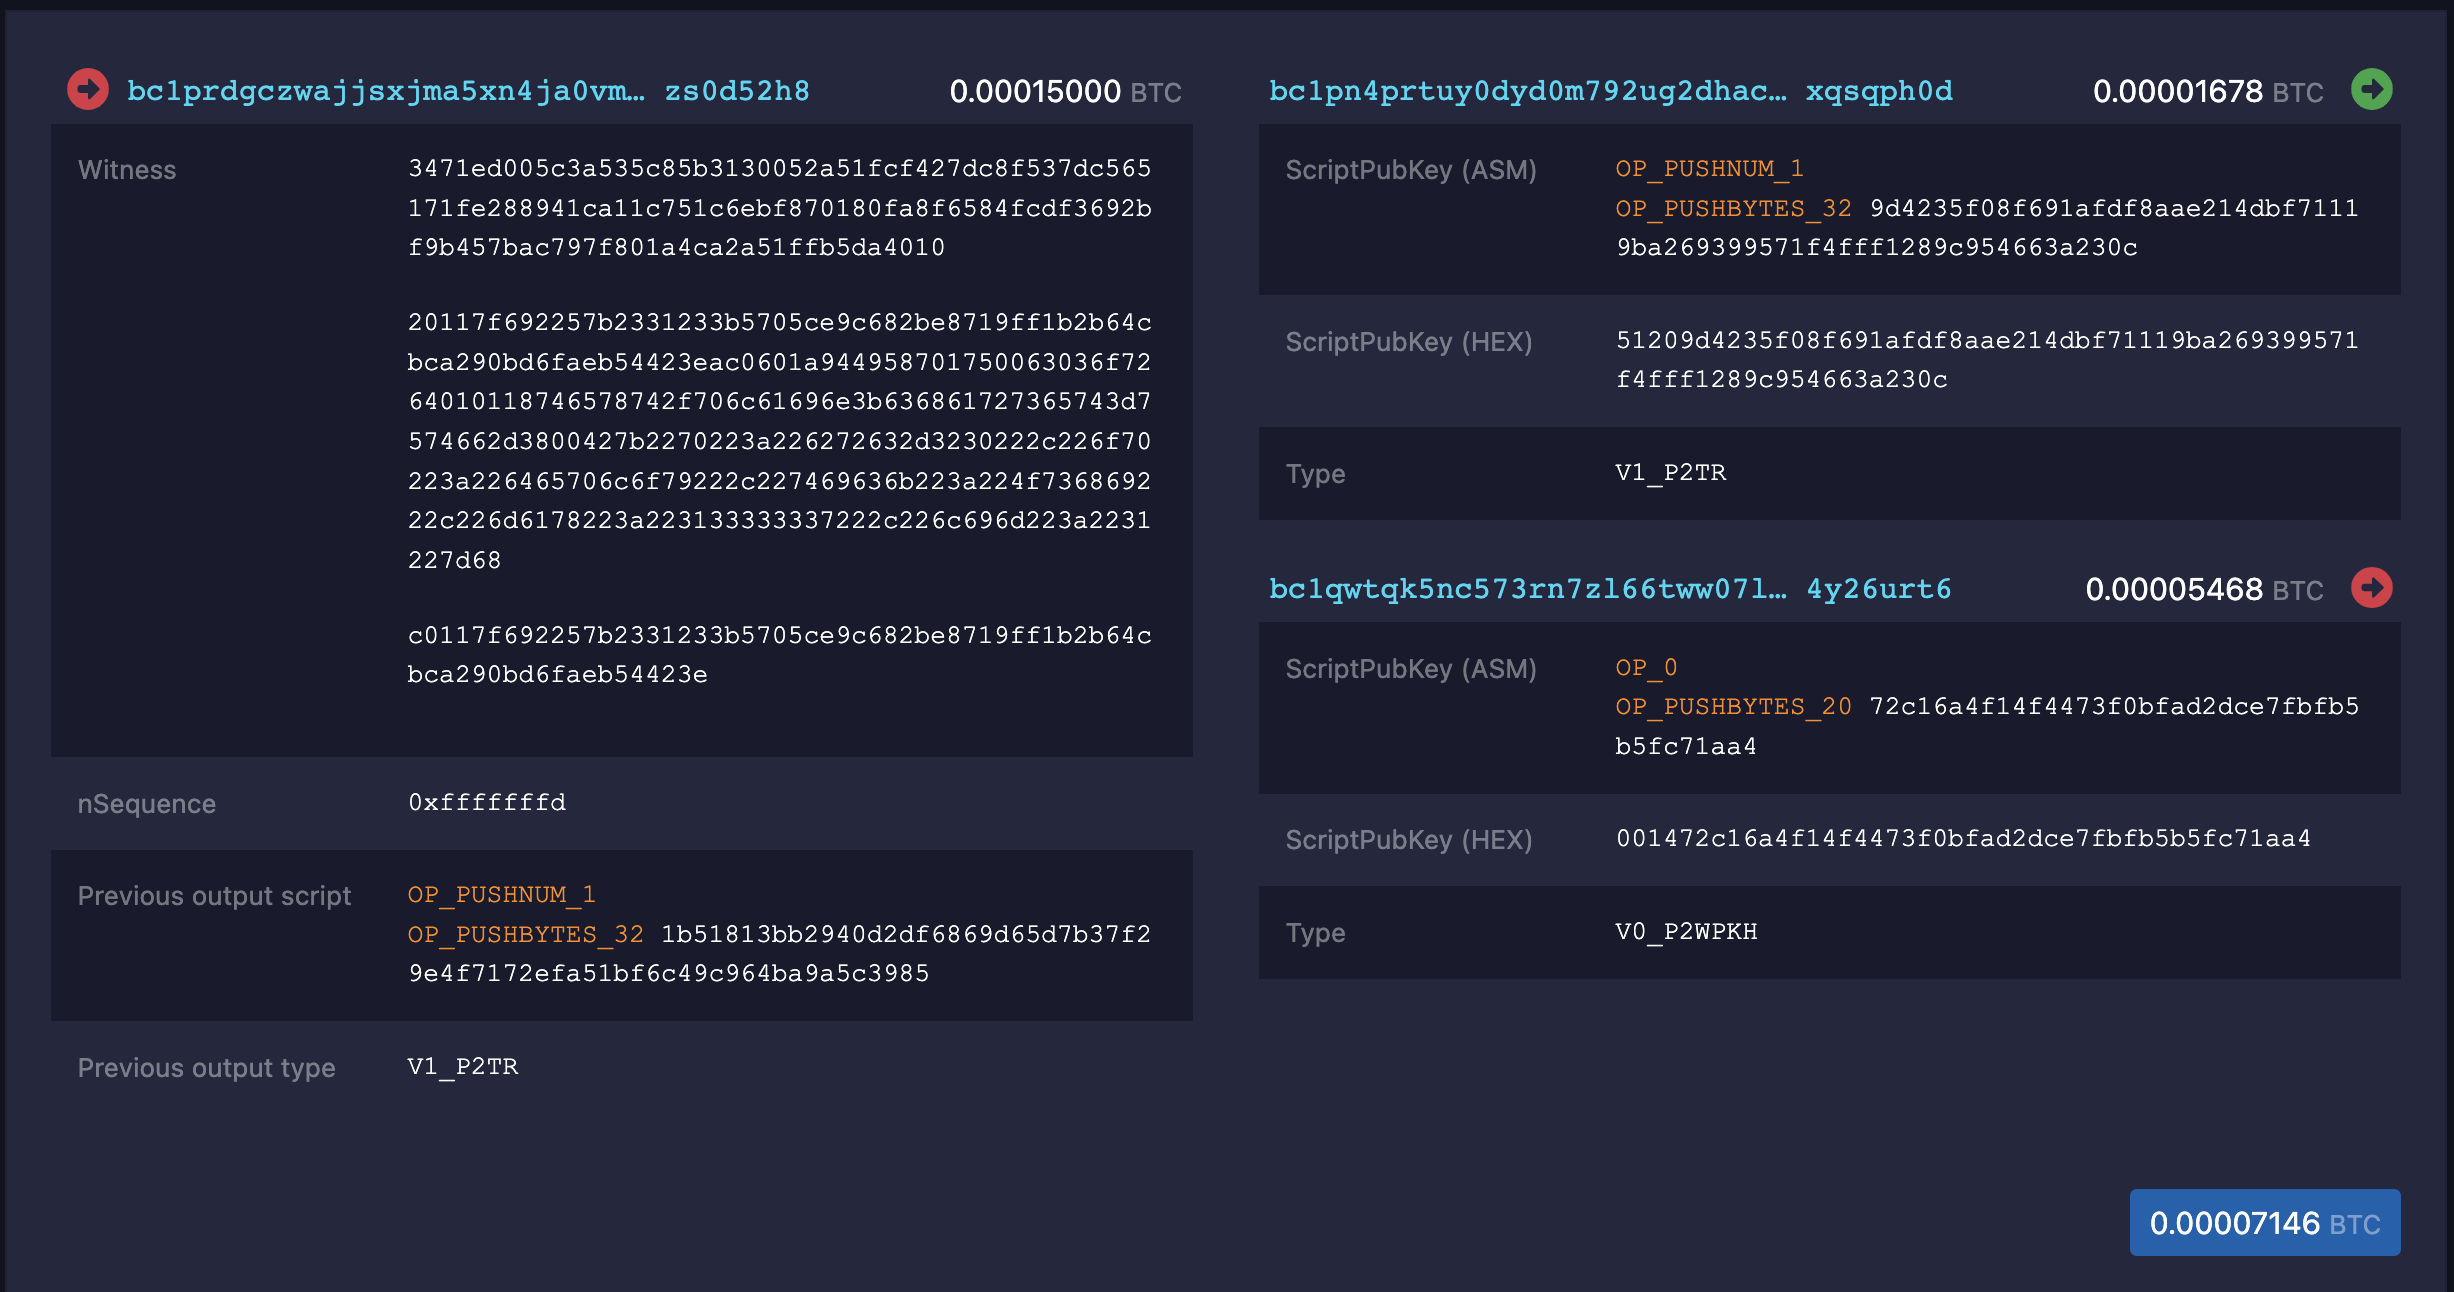
\includegraphics[width=\textwidth]{tx.png}
  \end{minipage}
  \hfill
  \begin{minipage}[b]{0.4\textwidth}
    \centering
    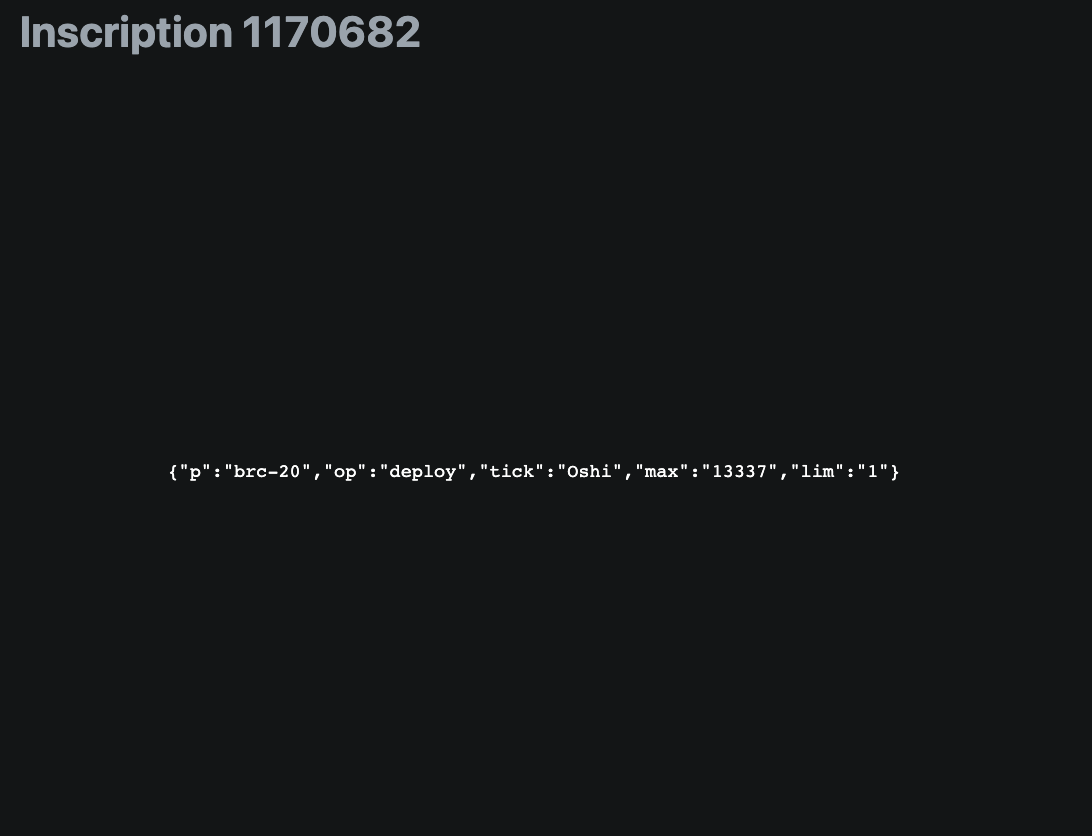
\includegraphics[width=\textwidth]{inscription.png}
  \end{minipage}
  \caption{\href{https://mempool.space/tx/940e8a6ec3943962c55fdd84809f3d878c6990da123cd3d02ae4769d3d86f3a6}{Bitcoin transaction} (left) \href{https://ordinals.com/inscription/940e8a6ec3943962c55fdd84809f3d878c6990da123cd3d02ae4769d3d86f3a6i0}{data inscribed} (right)}
\end{figure}

\item {\bf Data visualisation for on-chain data} \\
This is a real problem in blockchain ecosystem. \href{https://www.chainalysis.com/\#Products}{The Blockchain Data Platform - Chainalysis} makes several use of on-chain data visualisation. One great article that could be reviewed in this way is \cite{data-viz} which aims to give every tools to provide such visualisation. The master thesis of M. Kaandorp \cite{query-thesis} should also be regarded for its querying technics.\\
A basic example of what we can do is \url{mempool.space}. 
In the Decentralised Finance (DeFi) space data aggregation as \href{https://defillama.com/}{DeFi Lama} is very important. Professional tools can be used to create such aggregation about different protocols and with different utilities. Make a visual representation of these data can be a game changer in the blockchain realm.\\
With the development of  \href{https://ec.europa.eu/digital-building-blocks/code/projects/EBSI}{European Blockchain Service Infrastructure (EBSI)}, it can be a major problem for future industries and companies. 


\item {\bf Market data}\\ 
This is obviously a big deal for financial market especially in the case where this data are more or less easily available. There is a recent article which considered wash trade detection from on-chain liquidity data \cite{wash-trade}. This would begin to be a big research field when we know that Blackrock is arriving into the Bitcoin Market \href{https://www.reuters.com/technology/nasdaq-refiles-blackrocks-bitcoin-etf-application-with-sec-2023-07-03/}{Nasdaq refiles BlackRock's bitcoin ETF application with SEC}. \\
One major advantage of these data are to be more convenient than rough blockchain data \cite{finance-blch}. As shown in Lie, Xie et alt. \cite{deep-learning-blch} we can make implementation of deep learning to use more efficiently market data from blockchain. 

\item {\bf Data from mining}\\ 
Mining data have different aspects.\\ 
In one hand it's to mesure Bitcoin electricity consumption \cite{mining-elec, bitcoin-mining-elec} \href{https://ccaf.io/cbnsi/cbeci}{Cambridge Bitcoin Electricity Consumption Index (CBECI)}.\\ 
In another hand, it can be with many different use case for example in Zhu, Liu et alt. \cite{mining-data} they present the interest "to de-anonymize" transactions with making use of IP address from Bitcoin miners. The security of the network is depending on HashRate power \cite{security-btc} and we can link this data with market data as in Kubal et alt. \cite{price-security-btc} to learn more about the network.

\item {\bf Store and authenticate data} \\ 
The problem of data integrity is a real challenge in big data \cite{survey-bigdata-blockchain}. I need to learn more about data integrity to be able to give arguments about how the blockchain could help in this way. But in \cite{survey-bigdata-blockchain} we can find an array which summarises challenges that blockchain could solved in Big Data management.

\begin{figure}[h!]
\centering
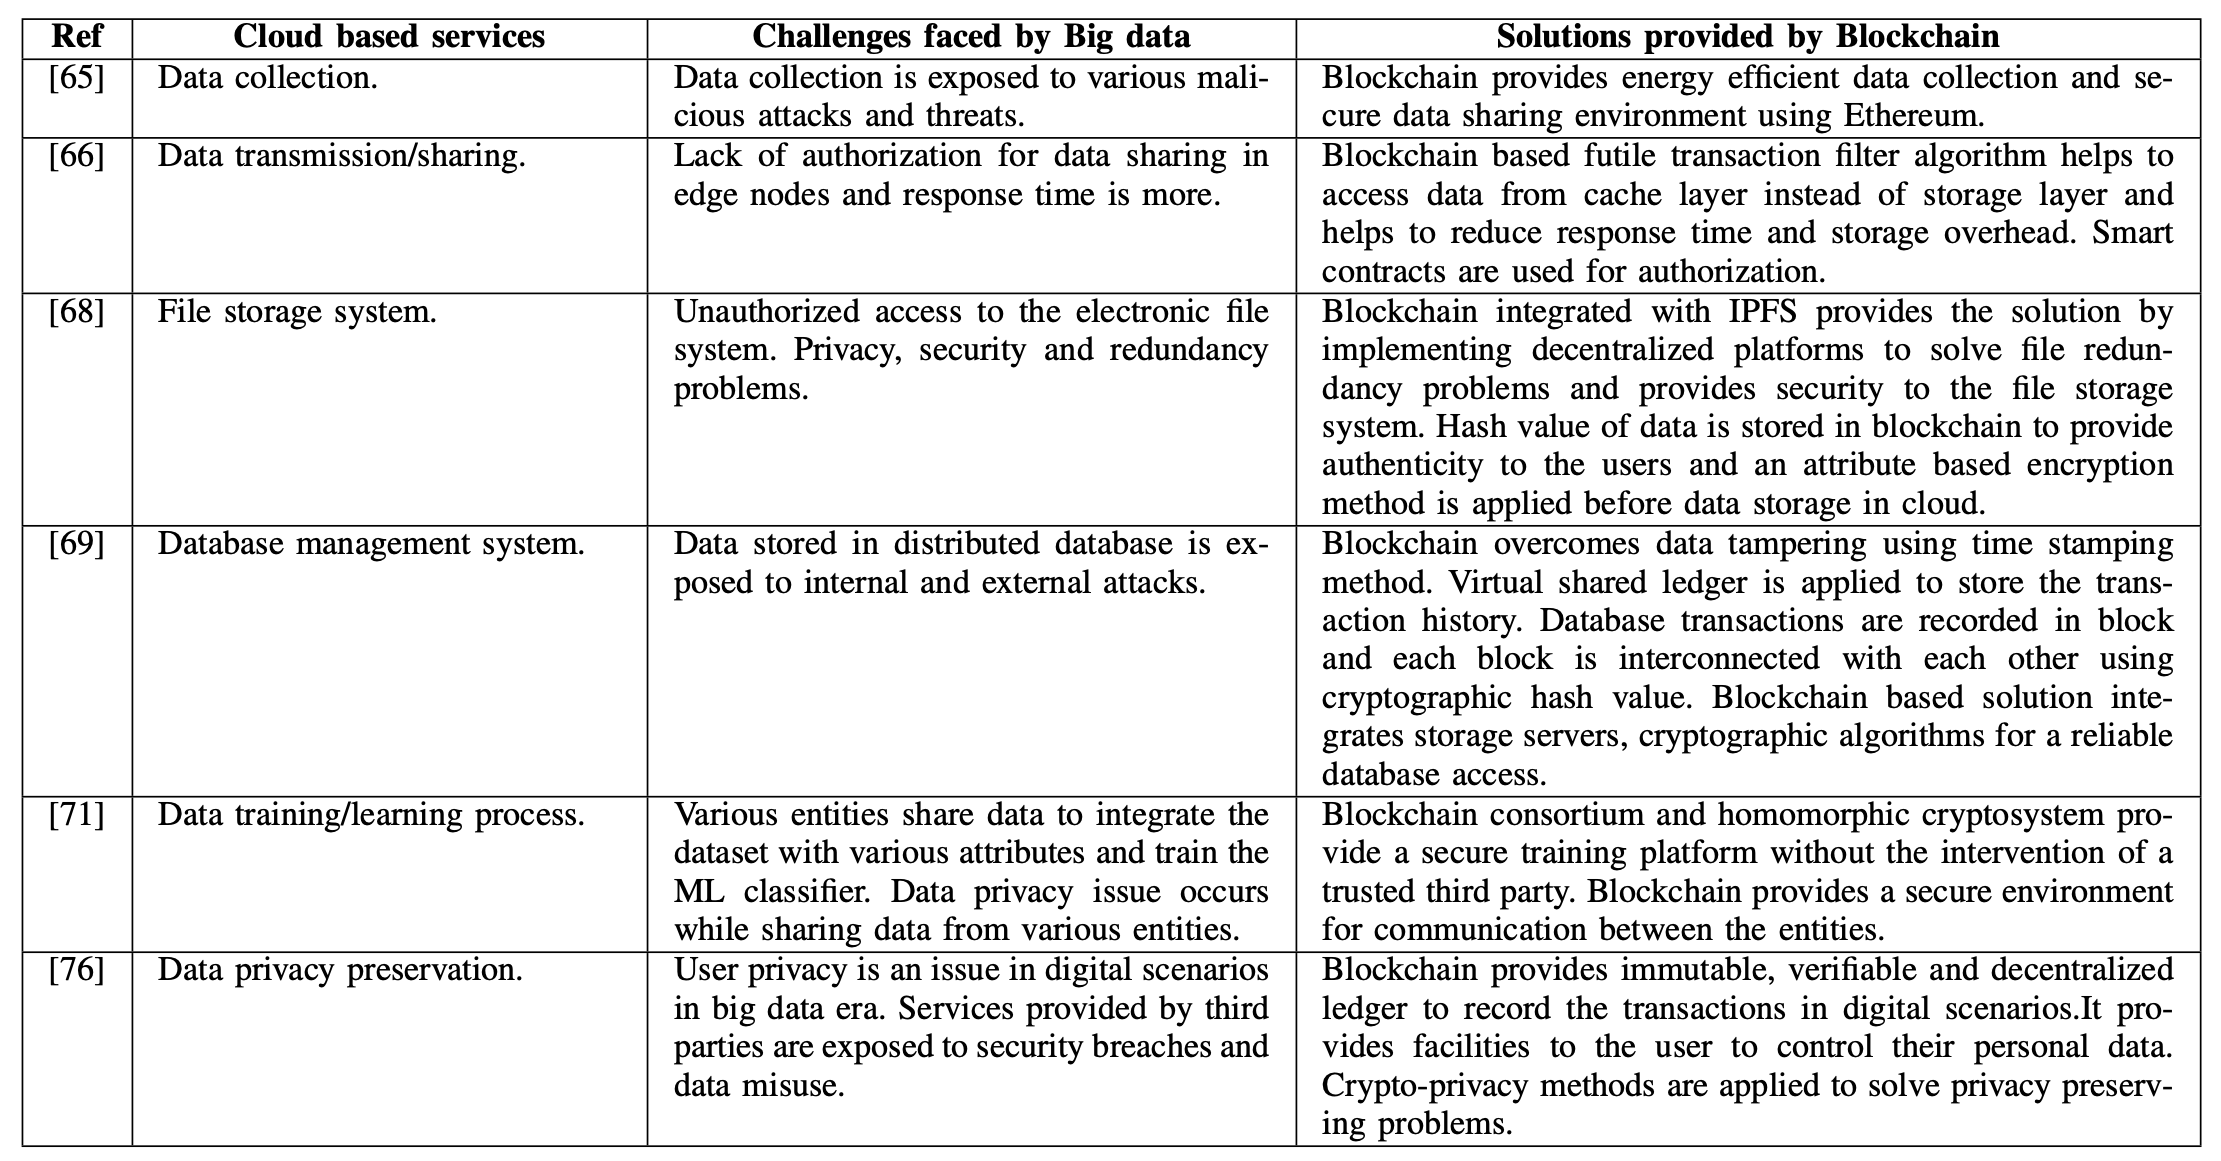
\includegraphics[scale=0.43]{solutions_blockchain_bigdata.png}
\caption{SERVICES PROVIDED BY CLOUD ENVIRONMENT FOR BIG DATA, CHALLENGES AND BLOCKCHAIN BASED SOLUTIONS.}

\end{figure}

\end{enumerate}

This list is not exhaustive and show what paths can be taken in data blockchain related problems.


\section{Some paths to do this ?}

It can be done in different ways but I think the most important to begin is to be able to retrieve any of data in any blockchain and provide studies about these data. It's the role of explorer and some research made several use of these explorers \cite{wash-trade}, but we need to go further and get data directly from blockchain.  
Especially, with the help of good parsers we can imagine to be able to retrieve and represent data in a quite short time with making use of tools purposed in \cite{data-viz}.

So the first step should be to make a deep study into Przytarski, Stach, Gritti et alt. \cite{query} especially from the state of the art section and a review of the only serious paper in this field Deepa, Pham et alt. \cite{survey-bigdata-blockchain}.\\
After this, we can try to purpose some experimentations of two types. \\
One with making use of \href{https://aws.amazon.com/blogs/database/access-bitcoin-and-ethereum-open-datasets-for-cross-chain-analytics/}{AWS tools}.\\ 
Another with the \href{https://github.com/ethereum/go-ethereum}{geth client} and blockchain directly on the machine where are doing experiments. The second proposal was made in the master thesis of M. Kaandorp \cite{query-thesis}, and should be analysed with taking attention on the recent update of \texttt{geth} \cite{geth} client. \\
Is it still interesting to do this ? Can we use this method and improve results with GraphQL native queries ?\\
A study about \href{https://en.wikipedia.org/wiki/Fog_computing}{fog computing} based on Sànchez, et alt. \cite{fogcomputing}, could be done to improve our previous results by taking profit of decentralisation and cloud computing tools.\\
 
After this work, try an integration of tools deployed on European blockchain frameworks (EBSI) could be a good application of the previous work.\\

As there is more or less a lack of research in this way, it should be possible to produce new results and be published. Moreover, many companies could make several use of these tools and financing these research should definitely be possible. 



\section{Conclusion}

Even though blockchain is fairly new \cite{whitepaper-btc} (2008), many things happened until now. Today, think about decentralised database is possible. Far to be effective now but possible. For many reasons using Bitcoin as a shared database is a really bad idea. But with tools develop by Europe (EBSI) it would be possible. 

And think about new standards and new opportunities should obviously be done by knowing what is existing today !

Moreover experiencing actual data management on Blockchain should be a good way to go in this direction. 

\newpage

\section*{Appendix}

\subsection*{EVM Schema}

\begin{figure}[h!]
\centering
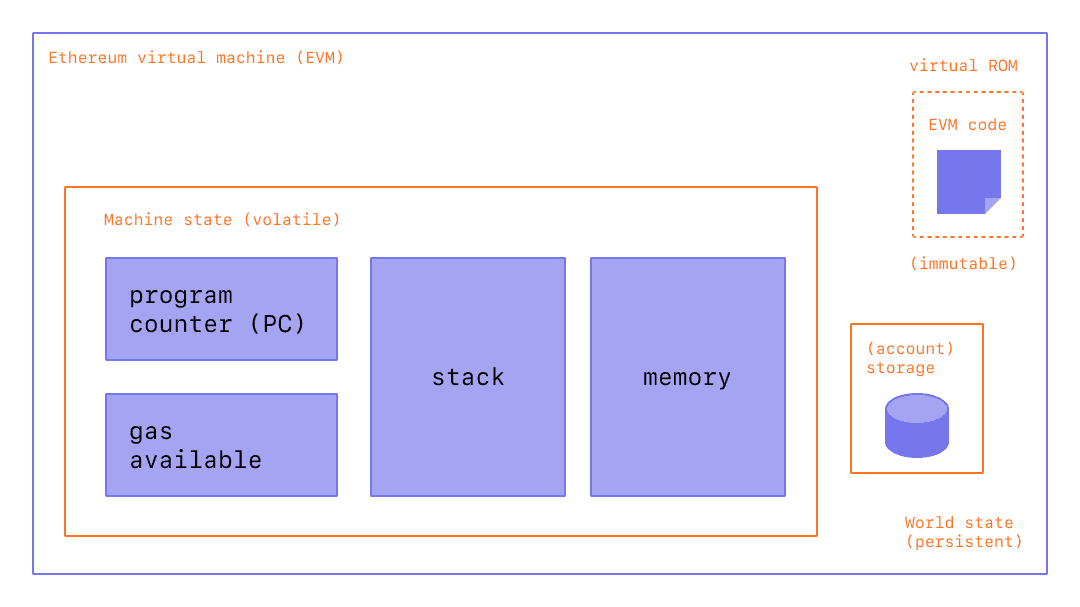
\includegraphics[scale=0.3]{evm.png}
\caption{EVM Schema \label{evm}}
\end{figure}



\subsection*{Bitcoin recent update\label{bitcoin}}

As we know the blockchain in the case of Bitcoin is a Distributed Ledger Technology (DLT) \cite{dlt}. It's mainly to store and transfer value all across the world with the only need of one address. But in a bitcoin transaction we can put a message. \\
With recent updates \href{https://github.com/bitcoin/bips/blob/master/bip-0141.mediawik}{Segregated Witness (Consensus layer)} (SegWit)\footnote{This BIP defines a new structure called a "witness" that is committed to blocks separately from the transaction merkle tree. This structure contains data required to check transaction validity but not required to determine transaction effects. In particular, scripts and signatures are moved into this new structure.
The witness is committed in a tree that is nested into the block's existing merkle root via the coinbase transaction for the purpose of making this BIP soft fork compatible. A future hard fork can place this tree in its own branch.
} we can push much more data in a Bitcoin transaction. This update allows a several major change in Bitcoin protocol : the Taproot update \cite{BIP341}\footnote{This proposal aims to improve privacy, efficiency, and flexibility of Bitcoin's scripting capabilities without adding new security assumptions. Specifically, it seeks to minimize how much information about the spendability conditions of a transaction output is revealed on chain at creation or spending time and to add a number of upgrade mechanisms, while fixing a few minor but long-standing issues.}.

Now there is a new protocol on top of Bitcoin to push data and retrieve it via an indexer. This protocol is called \href{https://docs.ordinals.com/}{Ordinals}.
With making use of an enveloppe we can post and retrieve easily data.

\begin{figure}[h!] 
\centering
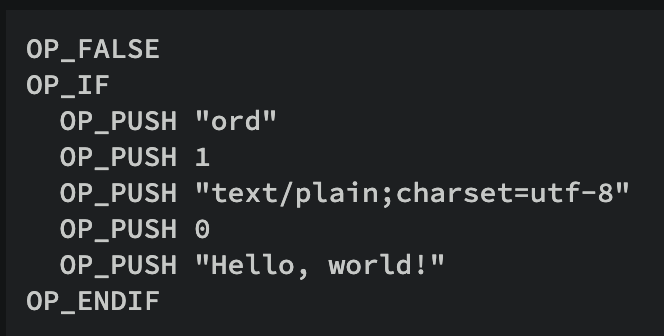
\includegraphics[scale=0.6]{ord_enveloppe.png}

\caption{Ordinal enveloppe's}
\end{figure}

This shown that we can build a basic database-like on top of Bitcoin. We can imagine how in a near future we would make use of Blockchain to allow many people to store and retrieve data. 

But it's a several change compare to our actual way to store data.












\newpage

\bibliographystyle{plain}  % Style de bibliographie (ici, le style "plain")
\bibliography{data_biblio} 



\end{document}



